%%% Класс документа
\documentclass[a4paper,14pt]{article}

%%% Работа с русским языком
\usepackage{cmap}					% поиск в PDF
\usepackage[warn]{mathtext}
\usepackage[T2A]{fontenc}			% кодировка
\usepackage[utf8]{inputenc}			% кодировка исходного текста
\usepackage[english,russian]{babel}	% локализация и переносы
\usepackage{mathtext} 				% русские буквы в формулах
\usepackage{csvsimple}              % for tabular from csv loading
\usepackage{indentfirst}            % indent after sections
%\usepackage{minipage}

%%% Дополнительная работа с математикой
\usepackage{amsmath,amsfonts,amssymb,amsthm,mathtools} % AMS
\usepackage{icomma} % "Умная" запятая: $0,2$ --- число, $0, 2$ --- перечисление

%%% Номера формул
%\mathtoolsset{showonlyrefs=true} % Показывать номера только у тех формул, на которые есть \eqref{} в тексте.
%\usepackage{leqno} % Немуреация формул слева

%%% Шрифты
\usepackage{euscript}	 % Шрифт Евклид
\usepackage{mathrsfs} % Красивый матшрифт

%%% Свои команды
\DeclareMathOperator{\sgn}{\mathop{sgn}}

%%% Перенос знаков в формулах (по Львовскому)
\newcommand*{\hm}[1]{#1\nobreak\discretionary{}
{\hbox{$\mathsurround=0pt #1$}}{}}

%%% Работа с картинками
\usepackage{graphicx}  % Для вставки рисунков
\graphicspath{{images/}{images2/}}  % папки с картинками
\setlength\fboxsep{3pt} % Отступ рамки \fbox{} от рисунка
\setlength\fboxrule{1pt} % Толщина линий рамки \fbox{}
\usepackage{wrapfig} % Обтекание рисунков и таблиц текстом

%%% Работа с таблицами
\usepackage{array,tabularx,tabulary,booktabs} % Дополнительная работа с таблицами
\usepackage{longtable}  % Длинные таблицы
\usepackage{multirow} % Слияние строк в таблице

%%% Теоремы
\theoremstyle{plain} % Это стиль по умолчанию, его можно не переопределять.
%\newtheorem{theorem}{Теорема}[section]
%\newtheorem{proposition}[theorem]{Утверждение}
 
%\theoremstyle{definition} % "Определение"
%\newtheorem{corollary}{Следствие}[theorem]
%\newtheorem{problem}{Задача}[section]
 
%\theoremstyle{remark} % "Примечание"
%\newtheorem*{nonum}{Решение}

%%% Программирование
\usepackage{etoolbox} % логические операторы

%%% Страница
\usepackage{extsizes} % Возможность сделать 14-й шрифт
\usepackage{geometry} % Простой способ задавать поля
	\geometry{top=25mm}
	\geometry{bottom=35mm}
	\geometry{left=35mm}
	\geometry{right=20mm}
	
%%% Колонтитулы
%\usepackage{fancyhdr}
 	%\pagestyle{fancy}
 	%\renewcommand{\headrulewidth}{0mm}  % Толщина линейки, отчеркивающей верхний колонтитул
 	%\lfoot{Нижний левый}
 	%\rfoot{Нижний правый}
 	%\rhead{Верхний правый}
 	%\chead{Верхний в центре}
 	%\lhead{Верхний левый}
 	% \cfoot{Нижний в центре} % По умолчанию здесь номер страницы
 	
%%% Интерлиньяж
%\usepackage{setspace}
%\onehalfspacing % Интерлиньяж 1.5
%\doublespacing % Интерлиньяж 2
%\singlespacing % Интерлиньяж 1

%%% Гиперссылки
\usepackage{hyperref}
\usepackage[usenames,dvipsnames,svgnames,table,rgb]{xcolor}
\hypersetup{				% Гиперссылки
    unicode=true,           % русские буквы в раздела PDF
    pdftitle={Заголовок},   % Заголовок
    pdfauthor={Автор},      % Автор
    pdfsubject={Тема},      % Тема
    pdfcreator={Создатель}, % Создатель
    pdfproducer={Производитель}, % Производитель
    pdfkeywords={keyword1} {key2} {key3}, % Ключевые слова
    colorlinks=true,       	% false: ссылки в рамках; true: цветные ссылки
    linkcolor=red,          % внутренние ссылки
    citecolor=green,        % на библиографию
    filecolor=magenta,      % на файлы
    urlcolor=cyan           % на URL
}

%%% Другие пакеты
\usepackage{lastpage} % Узнать, сколько всего страниц в документе.
\usepackage{soul} % Модификаторы начертания
\usepackage{csquotes} % Еще инструменты для ссылок
%\usepackage[style=authoryear,maxcitenames=2,backend=biber,sorting=nty]{biblatex}
\usepackage{multicol} % Несколько колонок
\usepackage{multirow} % Несколько строк

%%% Шрифты
%\renewcommand{\familydefault}{\sfdefault} % Начертание шрифта


%%% Работа с библиографией
%\usepackage{cite} % Работа с библиографией
%\usepackage[superscript]{cite} % Ссылки в верхних индексах
%\usepackage[nocompress]{cite} % 
%\usepackage{csquotes} % Еще инструменты для ссылок


%%% Tikz
\usepackage{tikz} % Работа с графикой
\usepackage{pgfplots} % Работа с pgf
\usepackage{pgfplotstable}
\usepackage{upgreek}

%%% Дополнительные пакеты для tikz
%\usepgfplotslibrary{dateplot} % Возможность подписания дат
\pgfplotsset{compat=1.5}
% \newcommand{\eqdef}{\stackrel{\mathrm{def}}{=}}
% \newcommand{\ryad}{\sum\limits^{\infty}_{k = 0}}

% \newcommand{\R}{\mathbb{R}}
% \newcommand{\N}{\mathbb{N}}
% \newcommand{\series}{\sum\limits_{k=1}^{\infty}}
% \newcommand{\useries}{\sum\limits_{k=1}^{\infty} u_k}
% \newcommand{\useriesl}{\sum\limits_{k=1}^{\infty} u_k < \infty}
% \newcommand{\useriese}{\sum\limits_{k=1}^{\infty} u_k = \infty}
% \newcommand{\auseries}{\sum\limits_{k=1}^{\infty} |u_k|}
% \newcommand{\auseriesl}{\sum\limits_{k=1}^{\infty} |u_k| < \infty}
% \newcommand{\auseriese}{\sum\limits_{k=1}^{\infty} |u_k| = \infty}
% \newcommand{\sn}{\sum\limits_{k=1}^{n} u_k}

% \renewcommand {\ge}{\geqslant}
% \renewcommand {\le}{\leqslant}
% \renewcommand {\geq}{\geqslant}
% \renewcommand {\leq}{\leqslant}
% \renewcommand {\epsilon}{\varepsilon}

\begin{document}
	
	%\newcommand{\HRule}{\rule{\linewidth}{0.7mm}} % Defines a new command for the horizontal lines, change thickness here
	
	\begin{center}
		\large\textbf{Московский Физико-Технический Институт}\\ % Name of your university/college
		\large\textbf{(государственный университет)}
	
		\vfill
		
		\Large Лабораторная работа по курсу общей физики № *labnum*\\[0.5cm] % Preambule of your document title
		
		
		\HRule
		\\[0.4cm]
		{ \huge \bfseries *name of your labwork*}% Title of your document
		\\[0.4cm] 
		\HRule
		\\[0.5cm]
		
		\ \\
	\textbf{\large Автор:} \\	
	\large *your name* *groupname*\\ % Your name and something more, your group num for example
		\vfill
		\hspace*{-0.8 cm}
\includegraphics[width=100 pt]{frkt_logo}\\ % logo of your  company/university/college
		\large Долгопрудный, 2021 % location and year
	\end{center}

\newpage
\setcounter{page}{2}
\fancyfoot[c]{\thepage}
\fancyhead[L] {Работа № *labnum*} % some information in page header
\fancyhead[R]{}
	
	\begin{comment}
	
	\section{Подготовка.}
	
	\noindent \textbf{В работе используются:} генератор импульсов, электронное реле, магазин сопротивлений, магазин емкостей, индуктивность, осциллограф, измеритель LCR.
	
	\noindent \textbf{Цель работы:} исследование зависимости периода свободных колебаний контура от емкости, зависимость логарифмического декремента затухания от сопротивления, определить критическое сопротивление и добротность контура, пронаблюдать затухающие колебания на фазовой плоскости.
	
	\hfill \break
	
	\noindent \textbf{Схема установки.}
	
	\begin{figure} [h!]
		\centering
		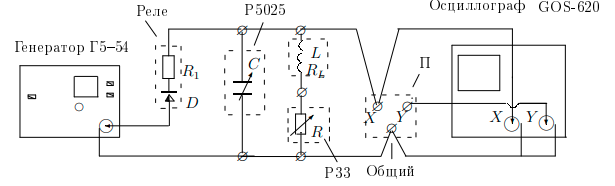
\includegraphics[scale = 0.75]{Схема установки для исследования свободных колебаний.png}
		\caption{Схема установки для исследования свободных колебаний}
	\end{figure}
	
	\hfill \break
	
	\noindent \textbf{Расчетные формулы.}
	
	\noindent Период колебательного контура.
	\begin{equation}
	T = 2 \pi \sqrt{LC}
	\end{equation}
	
	\noindent Частота колебательного контура.
	\begin{equation}
	\nu_0 = \frac{1}{2 \pi \sqrt{LC}}
	\end{equation}
	
	\noindent Критическое сопротивление.
	\begin{equation}
	R_{\text{кр}} = 2 \sqrt{\frac{L}{C}}
	\end{equation}
	
	\noindent Логарифмический декремент затухания.
	\begin{equation}
	\Theta = \frac{1}{n} \ln \frac{U_k}{U_{k + n}}
	\end{equation}
	
	\noindent Добротность.
	\begin{equation}
	Q = 2 \pi \frac{W}{\Delta W_T} = \frac{W}{\Delta W} = \frac{\pi}{\gamma T} = \frac{\omega_0 L}{R} = \frac{1}{\omega_0 CR} = \frac{1}{R} \sqrt{\frac{L}{C}}
	\end{equation}
	
	\newpage
	
	\end{comment}
	
	\section{Обработка данных.}
	
	\noindent Экспериментальным путем измерили период колебаний, при $R = 0$ $T = 340$ мкс; тогда частота колебаний составляет $\nu \approx 2941.18 Hz \approx 3 ~ \text{кГц} $.
	
	\hfill
	
	\noindent Используя формулу Томсона, вычислим индуктивность
	\begin{equation*}
		T = 2 \pi \sqrt{LC} \Rightarrow L = \frac{1}{C} \left(\frac{T}{2 \pi} \right)^2 = \frac{1}{2 \cdot 10^{-8}} \frac{3.4^2 \cdot 10^{-8}}{4 \pi^2} \approx 146.55 ~ \text{мГн}
	\end{equation*}
	
	\noindent Измерим индуктивность при помощи прибора ТЕТРОН-RLC200. Полученное значение -- $L = 143.47$ мГн.
	
	\noindent Примем расчетную погрешность 4\%; погрешность вычисления индуктивности $(\pm 5.74 ~ \text{мГн})$.
	
	\hfill
	
	\noindent \textbf{Вывод:} Таким образом, приходим к выводу, что полученные значения совпадают в пределах погрешности.
	
	\hfill
	
	\noindent Измерим зависимость $T^2(C)$; построим график данной зависимости.
	
	\begin{table}[h!]
		\begin{center}
			\begin{tabular}{|c|c|c|c|c|c|} \hline
				$C$ ($10^{-2}$ мкФ)   & 1     & 2      & 4      & 7      & 9 \\ \hline
				$T^2$ ($10^3$ мкс$^2$) & 57.6  & 115.6  & 230.4  & 409.6  & 518.4  \\ \hline
			\end{tabular}
		\end{center}
	\end{table}

	\noindent По графику проверим справедливость формулы Томсона.
	
	\begin{figure} [h!]
		\centering
		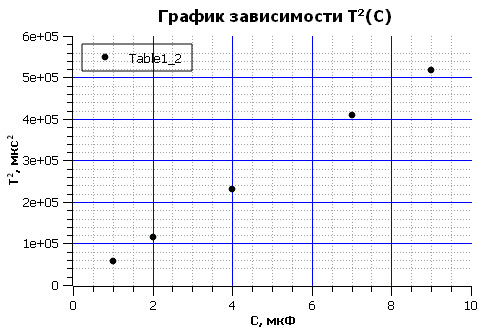
\includegraphics[scale = 1]{формулаТомсона.jpg}
	\end{figure}

	\noindent \textbf{Вывод:} график $T^2(C)$ представляет собой линейную зависимость, таким образом, приходим к выводу о справедливости формулы Томсона.
	
	\noindent Измерим зависимость логарифмического декремента затухания от сопротивления. 

	\begin{table} [h!]
		\begin{center}
			\begin{tabular}{|c|c|c|c|c|}
				\hline
				$R_{\text{внеш}}$, Ом  & $n$  & $U_1/U_n$ & $\theta$ & $Q$     \\ \hline
				0  & 23 & 2     & 0.03  & 104.6 \\ \hline
				2  & 21 & 2     & 0.033 & 95.15 \\ \hline
				4  & 20 & 2     & 0.034 & 92.35 \\ \hline
				6  & 19 & 2     & 0.036 & 87.22 \\ \hline
				8  & 17 & 2     & 0.041 & 76.59 \\ \hline
				10 & 25 & 3     & 0.044 & 71.36 \\ \hline
				12 & 24 & 3     & 0.046 & 68.26 \\ \hline
				15 & 28 & 4     & 0.049 & 64.08 \\ \hline
			\end{tabular}
		\end{center}
	\end{table}

	\noindent Вычислим теоретическое значение критического сопротивления.
	
	\begin{equation*}
		R_{\text{кр}} = 2 \sqrt{\frac{L}{C}} = 2 \sqrt{\frac{143.47 \cdot 10^{-3}}{2 \cdot 10^{-8}}} \approx  5356.68 \text{Ом}
	\end{equation*}
	
	\begin{equation}
		\theta = \gamma T = \frac{R}{2 L} 2 \pi \sqrt{L C} = R \pi \sqrt{\frac{C}{L}} = \frac{2 \pi}{R_{\text{кр}}}R
	\end{equation}
	
	\begin{equation}
		R = R_{\text{внеш}} + R_{\text{внутр}}
	\end{equation}
	
	\begin{equation}
		\theta = \frac{2 \pi}{R_{\text{кр}}} R_{\text{внеш}} + \frac{2 \pi}{R_{\text{кр}}} R_{\text{внутр}}
	\end{equation}
	
	\noindent Построим график зависимости $\theta(R)$ и выразим $R_{\text{внеш}}$ $R_{\text{внутр}}$.
	
	\begin{figure}[h!]
		\centering
		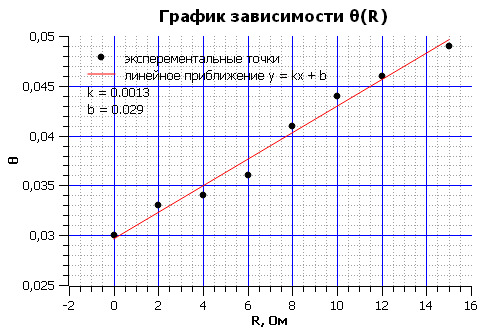
\includegraphics[scale = 1]{дикримент_сопротивление}
	\end{figure}
	
	\begin{equation*}
		\frac{2 \pi}{R_{\text{кр}}} = 0.0013 \Rightarrow R_{\text{кр}} \approx 4830.77 ~ \text{Ом}
	\end{equation*}
	
	\begin{equation*}
		\frac{2 \pi}{R_{\text{кр}}} R_{\text{внутр}} = 0.029 \Rightarrow R_{\text{внутр}} \approx 22.31 ~ \text{Ом}
	\end{equation*}
	
	\noindent \textbf{Вывод:} таким образом, с помощью графика зависимости $\theta(R)$ мы нашли значения внутреннего и критического сопротивления.
	
	\noindent Вычислим логарифмический декремент затухания по фазовой диаграмме.\\
	
	\begin{figure} [h!]
		\centering
		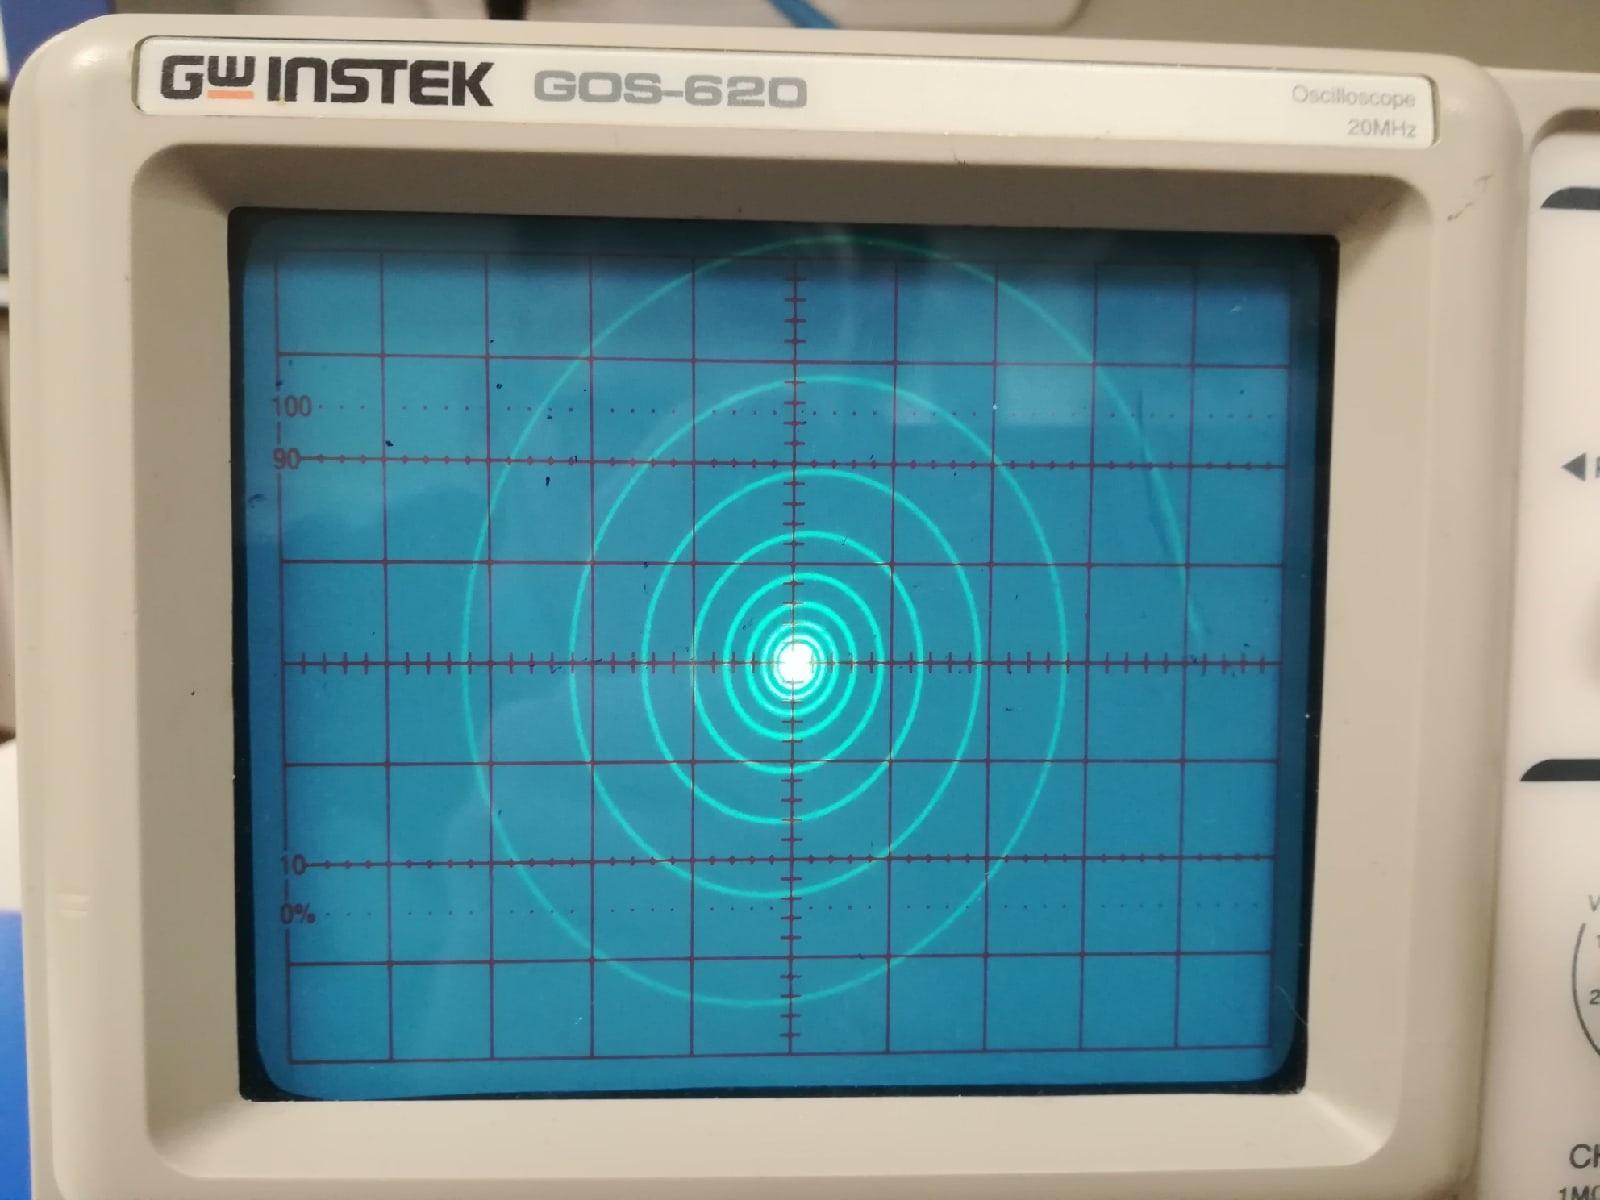
\includegraphics[scale = 0.16]{фазовая_диаграмма_рис1.jpg}
		\caption{Колебания на фазовой диаграмме R = 300 Ом}
	\end{figure}
	
	\begin{figure} [h!]
		\centering
		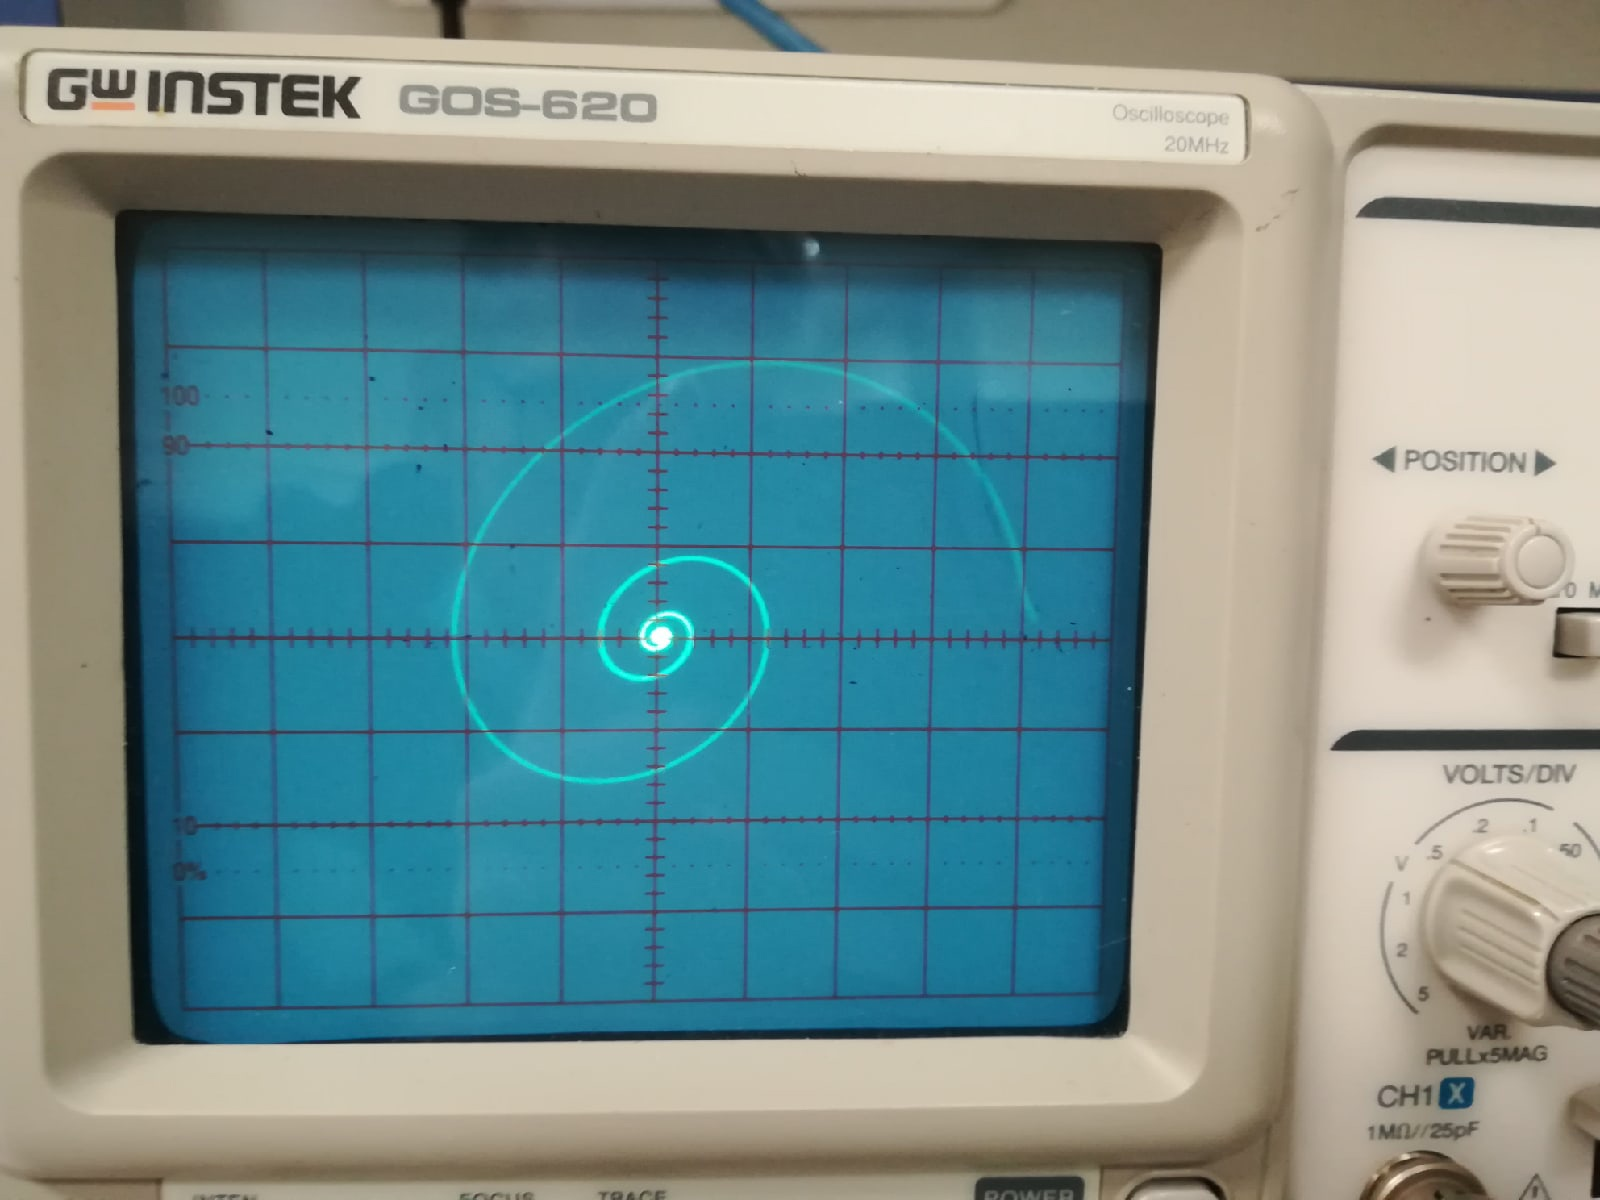
\includegraphics[scale = 0.16]{фазовая_диаграмма_рис2.jpg}
		\caption{Колебания на фазовой диаграмме R = 1 кОм}
	\end{figure}

	%\newpage

	\noindent Вычисления выполним по формуле:
	
	\begin{equation}
		\Theta = \frac{1}{n} \ln \frac{U_k}{U_{k + n}}
	\end{equation}
	
	\[ 300 ~ \text{Ом:} ~ \theta = \frac{1}{4} \ln \frac{14}{3} \approx 0.39 \]
	
	\[ 1 ~ \text{кОм:} ~ \theta = \ln \frac{6}{2} \approx 1.09 \]
	
\end{document}




